\documentclass{report}

\input{~/latex/template/preamble.tex}
\input{~/latex/template/macros.tex}

\title{\Huge{Graph and Tree Theory Notes}}
\author{\huge{Matt Warner}}
\date{\huge{}}
\pagestyle{fancy}
\fancyhf{}
\rhead{GRAPH AND TREE THEORY}
\lhead{\leftmark}
\cfoot{\thepage}
% \usepackage[default]{sourcecodepro}
% \usepackage[T1]{fontenc}
\usepackage{graphicx}
\usepackage{tikz}
\usepackage{pgfplots}
\usepackage{caption}
\usepackage{amsmath}
\pgfplotsset{compat=1.18}

\pgfpagesdeclarelayout{boxed}
{
  \edef\pgfpageoptionborder{0pt}
}
{
  \pgfpagesphysicalpageoptions
  {%
    logical pages=1,%
  }
  \pgfpageslogicalpageoptions{1}
  {
    border code=\pgfsetlinewidth{1.5pt}\pgfstroke,%
    border shrink=\pgfpageoptionborder,%
    resized width=.95\pgfphysicalwidth,%
    resized height=.95\pgfphysicalheight,%
    center=\pgfpoint{.5\pgfphysicalwidth}{.5\pgfphysicalheight}%
  }%
}

\pgfpagesuselayout{boxed}

\begin{document}
	\maketitle
\begin{LARGE}
		\textbf{\section{Trails, Paths, and Circuits}}
\end{LARGE}

\thmcon{
	\textbf{\underline{Definition}}
	\vspace{3mm}

Let $G$ be a graph, and let $v$ and $w$ be vertices in $G$.
\vspace{3mm}

A walk from $v$ to $w$ is a finite alternating sequence of adjacent vertices and edges of $G$. Thus a walk has the form

$$
v_0 e_1 v_1 e_2 \cdots v_{n-1} e_n v_n
$$

where the $v$ 's represent vertices, the $e$ 's represent edges, $v_0=v, v_n=w$, and for each $i=1,2, \ldots n, v_{i-1}$ and $v_i$ are the endpoints of $e_i$. The trivial walk from $v$ to $v$ consists of the single vertex $v$.
\vspace{3mm}
\begin{itemize}
  
\item A trail from $v$ to $w$ is a walk from $v$ to $w$ that does not contain a repeated edge.
\item A path from $v$ to $w$ is a trail that does not contain a repeated vertex.

\item A closed walk is a walk that starts and ends at the same vertex.

\item A circuit is a closed walk that contains at least one edge and does not contain a repeated edge.

\item A simple circuit is a circuit that does not have any other repeated vertex except the first and last.
\end{itemize}
}
\bigbreak \noindent 
\begin{center}
  \begin{table}[h]
    \centering
    \begin{tabular}{|l|c|c|c|c|}
        \hline
        & \textbf{Repeated} & \textbf{Repeated} & \textbf{Starts and Ends} & \textbf{Must Contain} \\
        & \textbf{Edge?} & \textbf{Vertex?} & \textbf{at Same Point?} & \textbf{at Least One Edge?} \\
        \hline
        Walk & allowed & allowed & allowed & no \\
        \hline
        Trail & no & allowed & allowed & no \\
        \hline
        Path & no & no & no & no \\
        \hline
        Closed Walk & allowed & allowed & yes & no \\
        \hline
        Circuit & no & allowed & yes & yes \\
        \hline
        Simple Circuit & no & \begin{tabular}{@{}c@{}}first and\\last only\end{tabular} & yes & yes \\
        \hline
    \end{tabular}
\end{table}
\end{center}
\bigbreak \noindent 
\ex{}{Determine which of the following walks are trails, paths, circuits, or simple circuits.

\begin{enumerate}
	\begin{multicols}{2}
	\item $v_1,e_1,v_2,e_3,v_3,e_4,v_3,e_5,v_4$
	\item $e_1,e_3,e_5,e_5,e_6$
	\end{multicols}
	\begin{multicols}{2}
	\item $v_2 v_3 v_4 v_5 v_3 v_6 v_2$
		\item $v_1e_1v_2e_1v_1$
	\end{multicols}
	\begin{multicols}{2}
		\item $v_2,v_3,v_4,v_5,v_6,v_2$
		\item $v_1$
		\end{multicols}
\end{enumerate}
}
\begin{figure}[ht]
	\centering
	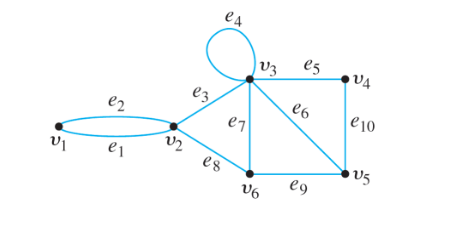
\includegraphics[width=0.5\textwidth]{figure1.png}
\end{figure}
\newpage

\pf{Soultion}

1. this walk is a Trail, since it does not contain any repeted edges.
\vspace{2mm}

2. This is just a walk and nothing else.
\vspace{2mm}

3. This walk is a Closed walk and is also a circuit, but not a simple circuit.
\vspace{2mm}

4. This is just a closed walk, it cant be a circuit since there is a repeated edge.
\vspace{2mm}

5. This is a closed walk, as well as a simple circuit.
\vspace{2mm}

6. This is a closed walk, as well as a trail, not a circuit becuase the walk does not contain any edges.
\bigbreak \noindent \bigbreak \noindent
\begin{LARGE}
	\textbf{\section{Subgraphs}}
\end{LARGE}
\bigbreak \noindent
\thmcon{
	\textbf{\underline{Defintion}}
	\vspace{3mm}
	
A graph $H$ is said to be a subgraph of a graph $G$ if, and only if, every vertex in $H$ is also a vertex in $G$, every edge in $H$ is also an edge in $G$, and every edge in $H$ has the same endpoints as it has in $G$.

}
\bigbreak \noindent \bigbreak \noindent
\ex{}{
	List all subgraphs of the graph $G$ with vertex set $\{v_1,v_2\}$ and edge set $\{e_1,e_2,e_3\}$, where the endpoints of $e_1$ are $v_1$ and $v_2$, the endpoints of $e_2$ are $v_1$ and $v_2$, and $e_3$ is a loop at $v_1$.
	\vspace{3mm}

	$G$ can be drawn as shown below.
	\vspace{2mm}


}

\begin{figure}[ht]
\centering
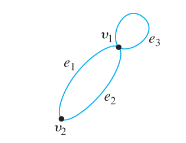
\includegraphics[width=0.3\textwidth]{ figure2.png }
\caption{$G$}
\end{figure}
\newpage

\noindent There are 11 subgraphs of $G$, which can be grouped according to those that do not have any edges, those that have one edge, those that have two edges, and those that have three edges.

\begin{figure}[ht]
\centering
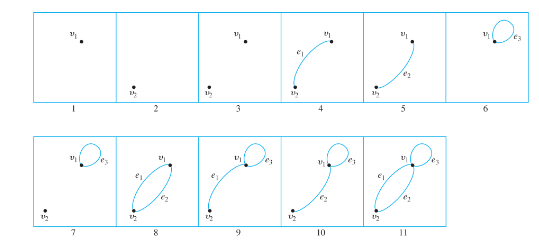
\includegraphics[width=0.5\textwidth]{ figure3.png }
\caption{Subgraphs of $G$}
\end{figure}
\bigbreak \noindent \bigbreak \noindent
\begin{LARGE}
	\textbf{\section{Connectedness}}
\end{LARGE}
\bigbreak \noindent
\thmcon{
	\textbf{\underline{Defintion}}
	\vspace{3mm}
	
	Let $G$ be a graph. Two \textbf{vertices, $v$ and $w$ of $G$ are connected} if, and only if, there is a walk from $v$ to $w$. 
	\vspace{2mm}
	
	The \textbf{graph $G$ is connected} if, and only if, given \textit{any} two vertices $v$ and $w$ in $G$, there is a walk from $v$ to $w$. Symbolically:
	\vspace{3mm}
	
	{\centerline{$G$ is connected $\longleftrightarrow$ $\forall$ vertices $v$ and $w$ in $G, \exists$ a walk from $v$ to $w$. }}
}
\bigbreak \noindent
\nt{
If you take the negation of this definition, you will see that a graph $G$ is \textit{not connected} if, and only if, there exists two vertices of $G$ that are not connected by any walk.}
\bigbreak \noindent \bigbreak \noindent
\ex{}{
	Which of the following graphs are connected?
	\vspace{3mm}

	The graphs are listed below
}
\begin{figure}[ht]
\centering
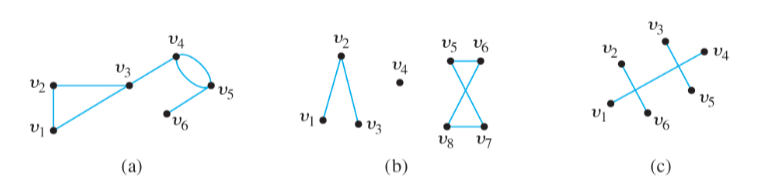
\includegraphics[width=0.8\textwidth]{ figure4.png }
\end{figure}

\pf{Solution}

Graph $A$ is connected \hspace{14mm} Graph $B$ is not connected \hspace{14mm} Graph $C$ is also not connected
\newpage

\begin{large}
 Some useful facts relating circuits and connectedness are collected in the following lenma. 
\end{large}
\bigbreak \noindent
\mlenma{}{
Let $G$ be a graph.
\vspace{2mm}

a. If $G$ is connected, then any two distinct vertices of $G$ can be connected by a path.
\vspace{2mm}

b. If vertices $v$ and $w$ are part of a circuit in $G$ and one edge is removed from the circuit, then there still exists a trail from $v$ to $w$ in $G$.
\vspace{2mm}

c. If $G$ is connected and $G$ contains a circuit, then an edge of the circuit can be removed without disconnecting $G$.
}
\bigbreak \noindent \bigbreak \noindent
\ex{}{
	Find all connected components of the following graph $G$.
}
\begin{figure}[ht]
\centering
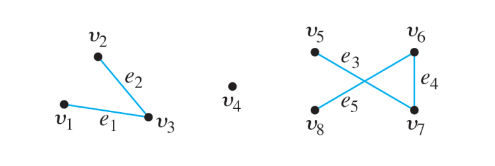
\includegraphics[width=0.7\textwidth]{ figure5.png }
\end{figure}
\pf{Solution}

\noindent $G$ has three connected components: $H_1,H_2$ and $H_3$ with vertex sets $V_1,V_2$, and $V_3$ and edge sets $E_1,E_2$, and $E_3$

\begin{center}
$$\begin{array}{ll}
V_1=\left\{v_1, v_2, v_3\right\}, & E_1=\left\{e_1, e_2\right\}, \\
V_2=\left\{v_4\right\}, & E_2=\varnothing, \\
V_3=\left\{v_5, v_6, v_7, v_8\right\}, & E_3=\left\{e_3, e_4, e_5\right\} .
\end{array}$$
\end{center}
\bigbreak \noindent \bigbreak \noindent 
\begin{LARGE}
	\textbf{\section{Euler Circuits}}
\end{LARGE}
\thmcon{
	\textbf{\underline{Defintion}}
	\vspace{3mm}

	Let $G$ be a graph. An Euler circuit for $G$ is a circuit that contains every vertex and every edge of $G$. That is, an Euler circuit for $G$ is a sequence of adjacent vertices and edges in $G$ that has at least one edge, starts and ends at the same vertex, uses every vertex of $G$ at least once, and uses every edge of $G$ exactly once.
}
\bigbreak \noindent
\thm{}{If a graph has a Euler circuit, then every vertex of the graph has positive even degree.
	\vspace{1mm}

	If some vertex of a graph has odd degree, then the graph does not have a Euler circuit
}
\newpage
\ex{}{
	\vspace{2mm}

	Show that the graph below does not have a Euler circuit.
}
\begin{figure}[ht]
\centering
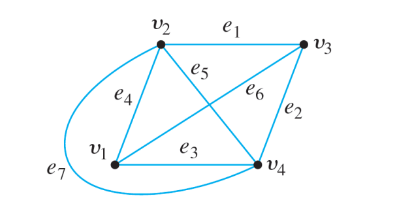
\includegraphics[width=0.5\textwidth]{ figure6.png }
\end{figure}

\pf{Solution}

\vspace{2mm}

	The vertices $v_1,$ and $v_3$ both have odd degrees (degree 3). So the graph cannot be a Euler circuit.
\bigbreak \noindent \bigbreak \noindent
\nt{
If a graph $G$ is connected and the degree of every vertex of $G$ is a postive even integer, then $G$ has a Euler circuit.
}
\bigbreak \noindent
\begin{large}
	\textbf{\subsection{Euler Trails}} 
\end{large}
\bigbreak \noindent 
\thmcon{
	\textbf{\underline{Defintion}}
	\vspace{3mm}

	Let $G$ be a graph, and let $v$ and $w$ be two distinct vertices of $G$. An Euler trail from $v$ to $w$ is a sequence of adjacent edges and vertices that starts at $v$, ends at $w$, passes through every vertex of $G$ at least once, and traverses every edge of $G$ exactly once.
}
\bigbreak \noindent 

\cor{}{Let $G$ be a graph, and let $v$ and $w$ be two distinct vertices of $G$. There is an Euler trail from $v$ to $w$ if, and only if, $G$ is connected, $v$ and $w$ have odd degree, and all other vertices of $G$ have positive even degree.}
\bigbreak \noindent \bigbreak \noindent \bigbreak \noindent 
\ex{}{
	The floor plan shown below is for a house that is open for public viewing. Is it possible to find a trail that starts in room $A$, ends in room $B$, and passes through every interior doorway of the house exactly once? If so, find such a trail.
}
\newpage
\begin{figure}[ht]
\centering
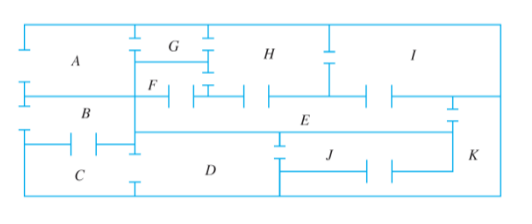
\includegraphics[width=0.5\textwidth]{ figure7.png }
\end{figure}

{\centerline{We can represent this floor plan as a graph:}}
\begin{figure}[ht]
\centering
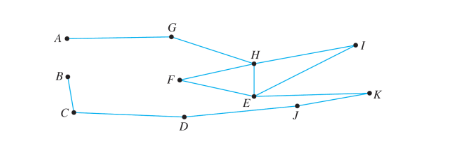
\includegraphics[width=0.5\textwidth]{figure8.png }
\end{figure}

Each vertex of this graph has an even degree except for $A$ and $B$, hence by Corollary 0.4.2 \\ \indent there is an Euler trail from $A$ to $B$ one such trail is

$$ A - G - H - F - E - I - H - E - K - J - D - C - B$$
\bigbreak \noindent \bigbreak \noindent 
\begin{LARGE}
	\textbf{\section{Hamiltonian Circuits}}
\end{LARGE}
\bigbreak \noindent
\thmcon{
	\textbf{\underline{Defintion}}
	\vspace{3mm}

	Given a graph $G$, a \textbf{Hamiltonian circuit} for $G$ is a simple circuit that includes every vertex of $G$. That is, a Hamiltonian circuit for $G$ is a sequence of adjacent vertices and distinct edges in which every vertex of $G$ appears exactly once, except for the first and the last, which are the same.
}
\bigbreak \noindent

\mprop{}{If a graph $G$ has a Hamiltonian circuit, then $G$ has a subgraph $H$ with the following properties:
	\vspace{2mm}	  

1. $H$ contains every vertex of $G$.
\vspace{2mm}

2. $H$ is connected.
\vspace{2mm}

3. $H$ has the same number of edges as vertices.
\vspace{2mm}

4. Every vertex of $H$ has degree 2 .}
\bigbreak \noindent \bigbreak \noindent
\newpage
\begin{large}
	\textbf{\section{Matrices}} 
\end{large}
\thmcon{
	\textbf{\underline{Defintion}}
	\vspace{3mm}

	Matrices are two-dimensional analogues of sequences.
	\vspace{2mm}

	They also are called two-dimensional arrays
	\vspace{4mm}

An $m \times n$ (read " $m$ by $n$ ") matrix A over a set $S$ is a rectangular array of elements of $S$ arranged into $m$ rows and $n$ columns:
\vspace{5mm}

	$\mathbf{A}=\left[\begin{array}{cccccc}
a_{11} & a_{12} & \cdots & a_{1 j} & \cdots & a_{1 n} \\
a_{21} & a_{22} & \cdots & a_{2 j} & \cdots & a_{2 n} \\
\vdots & \vdots & & \vdots & & \vdots \\
a_{i 1} & a_{i 2} & \cdots & a_{i j} & \cdots & a_{i n} \\
\vdots & \vdots & & \vdots & & \vdots \\
a_{m 1} & a_{m 2} & \cdots & a_{m j} & \cdots & a_{m n}
\end{array}\right] \leftarrow \text { ith row of } \mathrm{A}$
\vspace{5mm}

We write \textbf{A} = $(a_{ij})$
\vspace{5mm}

The $i$th row of A is 
$$
\left[\begin{array}{llll}
a_{i 1} & a_{i 2} & \ldots & a_{i n}
\end{array}\right]
$$
\vspace{3mm}

and the $j$th column of A is 
$$
\left[\begin{array}{c}
a_{1 j} \\
a_{2 j} \\
\vdots \\
a_{m j}
\end{array}\right]
$$
\vspace{6mm}

A matrix for which the numbers of row and columns are equal is called a \textbf{square matrix}
\vspace{5mm}

If $\mathbf{A}$ is a square matrix of size $n \times n$, then the main diagonal of $\mathbf{A}$ consists of all the entries $a_{11}, a_{22}, \ldots, a_{n n}$
}
\bigbreak \noindent
\begin{figure}[ht]
\centering
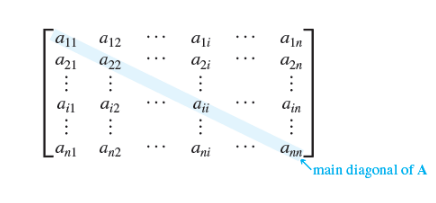
\includegraphics[width=0.55\textwidth]{ figure9.png }
\captionsetup{justification=centering,margin={-1cm,0cm}}
\caption{Square matrix diagonal}
\end{figure}
\newpage
\ex{}{
	The following is a 3 x 3 matrix over the set of integers.
	\vspace{3mm}

\begin{center}
	$\mathbf{A}=\left[\begin{array}{rrr}
	1 & 0 & -3 \\
	4 & -1 & 5 \\
	-2 & 2 & 0
\end{array}\right]$ 
\end{center}
\vspace{3mm}
\begin{enumerate}
	\item What is $a_{23}$, the entry in row 2 , column 3 ?
	\item What is the second column of $\boldsymbol{A}$ ?
	\item What are the entries in the main diagonal of $\mathbf{A}$ ?
\end{enumerate}
}
\pf{Solution}

\begin{large}
\begin{enumerate}
  
	\item $a_{23} = 5$
		\vspace{2mm}

	\item $\left[\begin{array}{r}
		0 \\
		-1 \\
		2
		\end{array}\right]$
		\vspace{2mm}

	\item $1, -1, 0$

\end{enumerate}  
\end{large}
\bigbreak \noindent \bigbreak \noindent
\begin{large}
	\textbf{\subsection{Matrices and Directed Graphs}}
\end{large}
\bigbreak \noindent
  
\begin{figure}[ht]
\centering
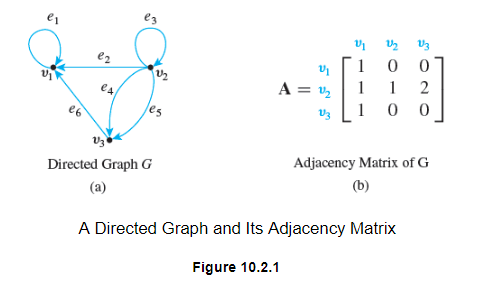
\includegraphics[width=0.5\textwidth]{ figure10.png }
\end{figure}
\bigbreak \noindent
\nt{As shown by the figure above, the adjacency matrix holds holds all the data for the directed graph, each entry in the matrix is either a $1$ or $0$, the entry is a 0 if the two vertices are not adjacent, and a 1 if they are adjacent, with the number increasing by the amount of edges that connect the vertices.}
\newpage
\ex{}{
	The two graphs show below are identical and differ only in the ordering of their vertices.
	\vspace{4mm}

	Find their adjacency matrices
}
\begin{figure}[ht]
\centering
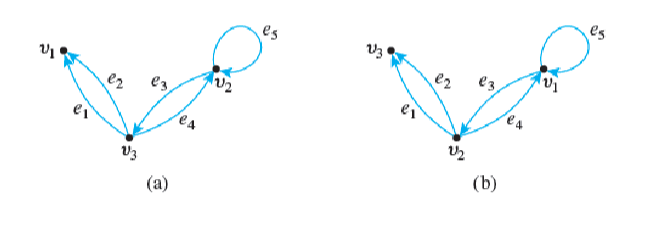
\includegraphics[width=0.7\textwidth]{ figure11.png }
\end{figure}

\pf{Solution}

\[
A = 
\begin{bmatrix}
0 & 0 & 0 \\
0 & 1 & 1 \\ 
2 & 1 & 0
\end{bmatrix}
\]

\end{document}


